%! suppress = MissingImport
You will now connect an external LED. An LED is a \textit{light emitting diode}, and like all diodes it allows current to flow only in one direction.
As shown in Figure~\ref{fig:led-annotated}, one lead on the LED is longer than the other, and this tells us which direction current will flow.
When we insert the LED into the circuit, power will flow from one of the \developmentboard's pins through the LED to ground.
Most LEDs have so little internal resistance that, unless current is otherwise limited, enough current will flow through the LED to destroy the semiconductor material.
The typical solution, which we will use, is to employ a \textit{current-limiting resistor}.
(If you look very closely at your \developmentboard, you will see a tiny surface-mount resistor next to each built-in LED.)

Figure~\ref{fig:led-diagram} shows a diagram of the components you will install for the LED output.

\begin{figure}
    \centering
    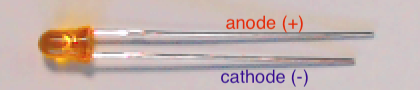
\includegraphics[height=2cm]{direct/led/led-annotated}
    \caption{The LED's longer lead connects to power; the shorter lead connects to ground.\label{fig:led-annotated}}
\end{figure}

\begin{figure}
    \centering
    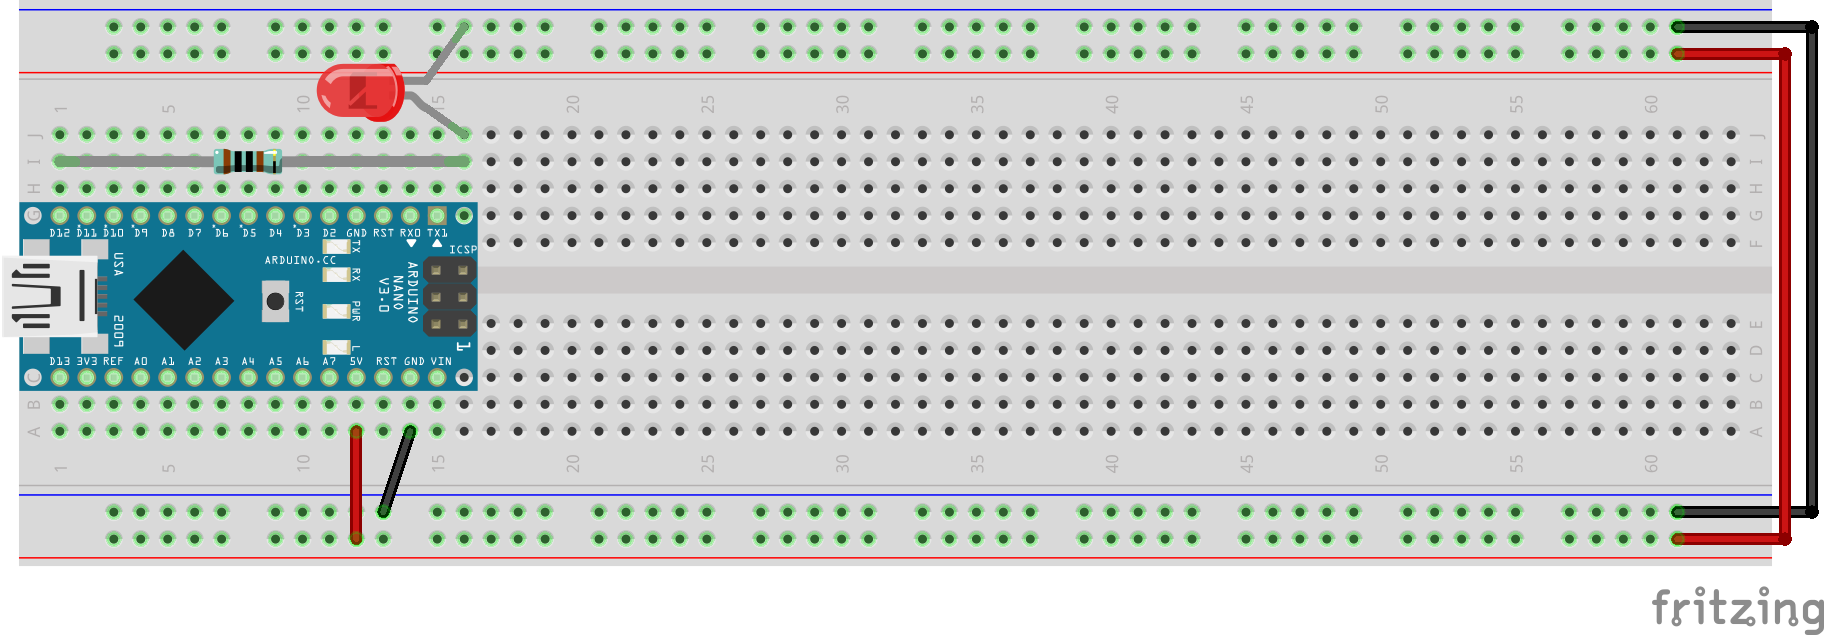
\includegraphics[width=0.9\textwidth]{fritzing_diagrams/led}
    \caption{Diagram of component assembly for LED output. \label{fig:led-diagram}}
\end{figure}

\begin{description}
    \checkoffitem{Take the 1k$\Omega$ resistor and place a right-angle bend in each lead about 0.4in (1cm) from the ends (we want the remaining length to be about 1.5in (3.8cm) -- you do not need to be exact;\footnote{If you want to try to be exact, you can use the breadboard's contact points to measure: they are 0.1in (2.54mm) apart.}
        the leads are flexible enough that you only need to be approximate) -- see Figure~\ref{fig:resistor-bent}.}
    \checkoffitem{Insert one of the resistor's leads into contact point \resistorcontactpointone\ (electrically connected to the \developmentboard's \ledpin\ pin in g1) and the other into contact point \resistorcontactpointtwo.}
    \checkoffitem{Gently press along the length of the resistor, causing the leads to deform slightly, until the resistor's height above the breadboard is about the same as the \developmentboard's printed circuit board.
        See Figure~\ref{fig:resistor-inserted}.}

    \checkoffitem{Take the LED and spread the leads apart slightly.}
    \checkoffitem{Insert the longer lead (the anode) in contact point \ledanodecontactpoint, and the shorter lead (the cathode) in the upper \ground.
        See Figure~\ref{fig:led-inserted}.}
\end{description}

\begin{figure}
    \centering
    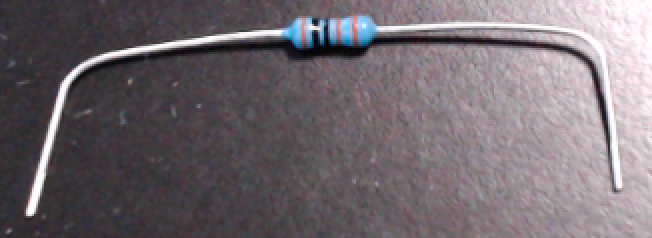
\includegraphics[height=2cm]{direct/led/resistor-bent}
    \caption{Bend the resistor's leads about 1cm from the ends.\label{fig:resistor-bent}}
\end{figure}

\begin{figure}
    \centering
    \subfloat[The resistor run between contact points \resistorcontactpointone\ and \resistorcontactpointtwo.]{
        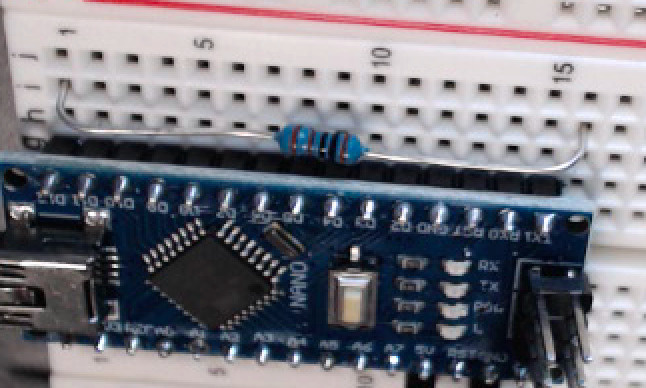
\includegraphics[width=0.65\textwidth]{direct/led/resistor-inserted}
        \label{fig:resistor-inserted}
    }
    \hfil
    \subfloat[The LED's longer lead is in contact point \ledanodecontactpoint, and its shorter lead is in the \ground.]{
        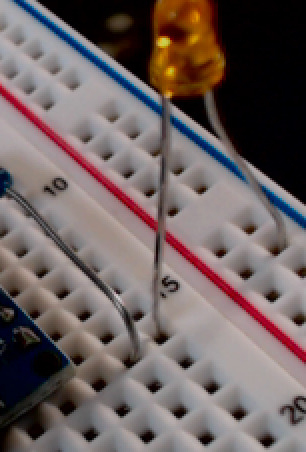
\includegraphics[width=0.25\textwidth]{direct/led/led-inserted}
        \label{fig:led-inserted}
    }
    \caption{Constructing the LED assembly.}
\end{figure}

When you have finished installing the external LED, there should be the electrical connections described in Table~\ref{tab:led}.
Read each of this and subsequent tables' rows as describing which electrical components are connected to which other components.
For example, the LED's anode is connected to the resistor's right lead;
the LED's cathode is connected to ground;
and the resistor's left lead is connected to the Arduino's ``\ledpin'' pin.

\begin{table}
    \begin{center}\begin{tabular}{||c|c|c|c||} \hline\hline
    LED lead    & Resistor lead & \developmentboard\ pin    & Pulled High/Low \\ \hline
    Anode       & Right         &           & \\
    Cathode     &               &           & \ground\ \\
                & Left          & \ledpin\  & \\ \hline\hline
    \end{tabular}\end{center}
    \caption{Electrical Connections for External LED.\label{tab:led}}
\end{table}

\checkpoint{installed the LED and its current-limiting resistor}

\begin{description}
    \checkoffitem{In the Arduino IDE, load \textit{MyBlink.ino}.}
%TODO: figure out how to generalize MyBlink
    \checkoffitem{In the \function{pinMode} and the two \function{digitalWrite} calls, replace the \lstinline{LED_BUILTIN} argument with \lstinline{12}:}
        \begin{lstlisting}
        void setup() {
          pinMode(12, OUTPUT);
        }

        void loop() {
          digitalWrite(12, HIGH);
          delay(250);   // or whatever value you used
          digitalWrite(12, LOW);
          delay(1500);  // or whatever value you used
        }
        \end{lstlisting}
    \checkoffitem{Re-connect the USB cable to your \developmentboard.}
    \checkoffitem{Compile the sketch and upload it to your \developmentboard.}
\end{description}
Now, instead of the built-in LED, the external LED that you installed will blink (Figure~\ref{fig:revisedblink}).

\begin{figure}
    \centering
    \animategraphics[autoplay,loop,height=4cm]{8}{direct/animations/revisedblink-}{0}{6}
    \caption{The revised \textit{MyBlink.ino} causes the external LED to blink.\label{fig:revisedblink}}
\end{figure}

